\documentclass[man, 12pt, floatsintext]{apa6}
\usepackage{amsmath, amsthm, amssymb}

\newtheorem{theorem}{Theorem}
\newtheorem{lemma}{Lemma}
\newtheorem{proposition}{Proposition}
\newtheorem{corollary}{Corollary}
\theoremstyle{definition}
\newtheorem{assumption}{Assumption}
\theoremstyle{remark}
\newtheorem{remark}{Remark}
\usepackage[american]{babel}
\usepackage{csquotes}
\usepackage{graphicx}
\usepackage{float}
\usepackage{caption}
\usepackage{subfigure}
\usepackage[style=apa,sortcites=true,sorting=nyt,backend=biber]{biblatex}

\AtEveryBibitem{
  \clearfield{month}
}
\DeclareLanguageMapping{american}{american-apa}

\DeclareSourcemap{
  \maps[datatype=bibtex]{
    \map{
      \step[fieldsource=url,
        notmatch=\regexp{wiki},
      final=1]
      \step[fieldset=urldate, null]
    }
  }
}

\addbibresource{ref.bib}

\title{Your Title}
\shorttitle{Short Title}
\author{Your Name}
\affiliation{Your Affiliation}

% \affiliation{Psychology Department$^{1}$, Computer Science Department$^{2}$, Center for Cognitive Science$^{3}$, Rutgers University--New Brunswick; Princeton Neuroscience Institute$^{4}$, Psychology Department$^{5}$, Computer Science Department$^{6}$, Princeton University}

\abstract{}
\keywords{}
\authornote{}

\begin{document}
\setlength{\parindent}{20pt}

\maketitle
\section{Derivation}

\noindent We are interested  in deriving the simplest model of learning which generates a spacing effect. For the current work, we consider the simple case of two repeated study sessions for the same material, followed by a delayed memory test. Set $y$ as the study separation time between study 1 and study 2 and $x$ as the test delay. The spacing effect can be described simply: the optimal lag between study sessions increases as the delay period of the test increases (Cepeda et al. 2008).

\begin{figure}
  \centering
  \includegraphics[width=0.60\linewidth]{cepeda.png}
  \caption{Results from a meta-analysis by Cepeda et al. (2008) demonstrating that the optimal study lag is approximately a linear function of the test delay on a log-log plot}\label{fig:cepeda}
\end{figure}

Consider a generic memory model with the following form:

\textbf{(1) Delta learning rule:}  When studying an item, a new trace is formed of the memory strength:
\begin{equation}
  B_{new} =\delta (B_{max} - B_{current}),
\end{equation}

\noindent where $B_{max} = 1$, $\delta$ is the learning rate ($0 < \delta < 1$), and $B_{current}$ is the summed strength of memory traces formed during previous repetitions of the item. Thus, after the very first occurrence of an item, its memory trace has strength $B_1 = \delta$.

\textbf{(2) Trace-specific forgetting:} The strength of each memory trace decreases independently as a monotonic function of time. Two standard such functions are an exponential decay and a power-based decay:
\begin{equation}
  \begin{aligned}
    f_{power}(t) &= {(1+t)}^{-\gamma} \\
    f_{exp}(t) &= e^{-\gamma t},
  \end{aligned}
\end{equation}

\noindent where $f(0)=1$ and $\gamma > 0$ and each memory trace decays independently as a function of time since its formation.

At any point in time, the summed memory strength is the sum of each trace weighted by its decay function:
\begin{equation}
  B_{current} = \sum_{k=1}^{n} B_k f(t_k),
\end{equation}

\noindent with $k$ being the k-th study repetition and $t_k$ is the time elapsed since.

In the special case with two study repetitions separated by an interval $y$ and where memory is tested \textit{x} units of time after the second session, we have the overall memory strength $B$ at test is a sum of the two memory traces after forgetting:
\begin{equation}\label{eq:B}
  \begin{aligned}
    B(x,y) &= B_{1} f(x+y) + B_{2} f(x)\\
    &= B_{1} f(x+y) + \delta (1 - B_{1} f(y)) f(x)\\
    &= \delta f(x+y) + \delta f(x) - \delta^2 f(x) f(y)\\
  \end{aligned}
\end{equation}

To capture the spacing effect, we are interested in deriving the optimal study separation $y$ that maximizes the memory strength B when the test delay $x$ is fixed. An optimal y that is a monotonically increasing function of x is possible only when the $B(x,y)$ is a convex function of y that has a real solution $y > 0$ to the system of equations involving its first two derivatives:
\begin{equation}
  \frac{dB}{dy} = 0  ,\,\, \frac{d^2B}{dy^2} < 0
\end{equation}

We get the general form of the derivatives from (4):
\begin{equation}
  \begin{aligned}
    \frac{dB}{dy} &= \delta f'(x+y) - \delta^2 f(x) f'(y) \\
    \frac{d^2B}{dy^2} &= \delta f''(x+y) - \delta^2 f(x) f''(y)
  \end{aligned}
\end{equation}

Since $0 < \delta < 1$, we can simplify them and have this final system of equations which a model with a spacing effect must satisfy:
\begin{equation}
  \begin{aligned}
    & f'(x+y) - \delta f(x) f'(y) = 0\\
    & f''(x+y) - \delta f(x) f''(y) < 0
  \end{aligned}
\end{equation}

\subsection{Exponential vs power-based decay}

Consider first the exponential-based decay with $f(x) = e^{-\gamma x}$:
\begin{equation}
  \begin{aligned}
    \delta^{-1}\frac{dB}{dy} &= \frac{d}{dy} e^{-\gamma(x+y)} - \delta e^{-\gamma x} \frac{d}{dy}e^{-\gamma y} \\
    &= -\gamma e^{-\gamma(x+y)} + \delta \gamma e^{-\gamma (x+y)} \\
    &= (\delta-1) \gamma e^{-\gamma (x+y)}\\
    \delta^{-1}\frac{d^2 B}{dy^2} &= - (\delta-1) \gamma^2 e^{-\gamma (x+y)}\\
  \end{aligned}
\end{equation}

Since the learning rate $\delta$ is strictly less than 1, then $(\delta-1) \gamma e^{-\gamma (x+y)} < 0$ and $- (\delta-1) \gamma^2 e^{-\gamma (x+y)} > 0$. The negative first derivative means that memory strength $B$ will always be highest when y is minimal and there is no spacing between the study items.

Now consider the power-based decay with $f(x) = (1+x)^{-\gamma}$
\begin{equation}
  \delta^{-1}\frac{dB}{dy} = -\gamma (x+y+1)^{-\gamma-1} + \delta \gamma(x+1)^{-\gamma} (y+1)^{-\gamma-1}
\end{equation}

Setting $\frac{dB}{dy}=0$, we have:
\begin{equation}
  (x+y+1)^{-\gamma-1} = \delta(x+1)^{-\gamma} (y+1)^{-\gamma-1}
\end{equation}

Both sides are positive, so set $r = -\frac{1}{\gamma+1}$, $-\gamma r = 1+r$, and raise each side to $r$ degree:

\begin{equation}
  \begin{aligned}
    ((x+y+1)^{-\gamma-1})^{r} &= (\delta(x+1)^{-\gamma} (y+1)^{-\gamma-1})^{r} \\
    x+(y+1) &= \delta ^{r} (x+1)^{1+r} (y+1) \\
    x &= (y+1)(\delta ^{r} (x+1)^{1+r}-1) \\
    y + 1 &= \frac{x}{\delta ^{r} (x+1)^{r+1}-1}
  \end{aligned}
\end{equation}

To simplify the expression, denote $\tilde{y} = y+1$ and $\tilde{x}=x+1$, the study and test lag offset by 1. Recognize also that $\delta^r = \delta^{-\frac{1}{\gamma+1}} \geq 1$ is a scaling constant that depends on the learning rate and the decay rate, so just replace it with a combined constant $\alpha > 1$. :
\begin{equation}\label{eq:closedform}
  \tilde{y} = \frac{\tilde{x}-1}{\alpha \tilde{x}^{\frac{\gamma}{1+\gamma}}-1}
\end{equation}

Since the exponent of $\tilde{x}$ in the denominator is $\gamma/(1+\gamma) < 1$, as the test lag x increases, so does the optimal study lag $y$.

Figures below show the optimal offset study gap $\tilde y$ in days as a function of offset test delay in days (both measures offset by 1 second as described above). First figure is on the native linear scale, while second figure is on a log10-log10 scale. Both parameters affect the position of the optimal line, but do not change the qualitative results. Increasing the learning during both study sessions makes the optimal study gap longer for the same test delay, although the effect is modest. The forgetting rate has more dramatic effects, but again it just shifts the intercept on the log-log scale. Neither parameter changes the shape of the optimal y as a function of x.

With the exception of $\gamma = 0.01$, all optimal lines are below the diagonal line, meaning that the optimal study gap is less than the test day for most parameter combinations. We included the $0.01$ decay rate condition to explore the extremes of the model - that said, it is not a reasonable parameter value and it is far from the range typically used  in power-based decay forgetting functions (REFS). All parameter values reproduce the general data pattern from Cepeda (2008). Particular parameter values can be chosen for a perfect fit to the empirical regression line, if desired.

\begin{figure}
  \centering
  \includegraphics[width=1\linewidth]{figures/f1_spacing_parameters_linear.png}
  \caption{Enter Caption}\label{fig:spacing-linear}
\end{figure}

\begin{figure}
  \centering
  \includegraphics[width=1\linewidth]{figures/f2_spacing_parameters_log_log.png}
  \caption{Enter Caption}\label{fig:spacing-loglog}
\end{figure}

\section{Generalization: Which Learning and Forgetting Functions Produce the Empirical Spacing Profile?}\label{sec:general}

The delta rule with power-law decay is one instance of a much larger model family. In this section we replace both ingredients by arbitrary functions and ask which of the results above are load-bearing properties of those particular choices and which are general theorems. To make the generalization transparent we switch notation: let $a$ denote the inter-study interval (previously $y$), $b$ the retention interval between the second study and the test (previously $x$), $g$ the learning function, and $f$ the forgetting function. A single study of an unknown item lays down a trace of strength $g(0)$; restudying an item whose currently retrieved strength is $s$ lays down a new, independently decaying trace of strength $g(s)$. The delta rule is the special case $g(s) = \delta(1-s)$. Keeping the multiplicative strength--forgetting form and the independent decay of the two traces, the retrieved strength at test is
\begin{equation}\label{eq:S}
  S(a,b) \;=\; g_0\, f(a+b) \;+\; g\!\big(g_0 f(a)\big)\, f(b), \qquad g_0 := g(0),
\end{equation}
which reduces to Equation~\ref{eq:B} under the delta rule. Throughout, $a^*(b)$ denotes a maximizer of $a \mapsto S(a,b)$ for a fixed retention interval $b$.

The empirical profile we want to explain --- the pattern in the Cepeda et al.\ (2008) meta-analysis summarized in Figure~\ref{fig:cepeda} --- consists of four properties:
\begin{itemize}
  \item[P1.] (\textit{Spacing effect.}) For all but possibly the shortest retention intervals, some spacing strictly beats massed restudy: $a^*(b) > 0$, with an interior optimum.
  \item[P2.] (\textit{Monotonicity.}) The optimal lag increases with the retention interval.
  \item[P3.] (\textit{Log-log linearity and sublinearity.}) $\log a^*$ is approximately linear in $\log b$ with slope less than 1, so the optimal lag grows without bound but the ratio $a^*/b$ falls.
  \item[P4.] (\textit{Robustness.}) Parameter changes shift the optimal-lag line but not its shape or slope.
\end{itemize}
The theorems below characterize, for essentially arbitrary $(g,f)$, exactly which ingredient produces each property. In brief: P1 requires \emph{encoding suppression} ($g$ decreasing) and puts a threshold on the hazard of forgetting; P2 is controlled by the forgetting function alone, through a sign rule that exponential decay violates on a knife edge; P3 and P4 are universal consequences of power-law-type forgetting, with a slope determined by $f$ (and only degenerately by $g$).

\subsection{Setup}

\begin{assumption}[Forgetting]\label{ass:f}
$f:[0,\infty)\to(0,1]$ is twice continuously differentiable with $f(0)=1$, $f'<0$, and $f(t)\to 0$ as $t\to\infty$. Define the \emph{hazard} $h(t) := -f'(t)/f(t) > 0$, the \emph{momentary forgetting rate} $m(t) := -f'(t) > 0$, and the \emph{proportional decay rate of the forgetting rate} $\lambda(t) := -m'(t)/m(t) = h(t) - (\log h)'(t)$.
\end{assumption}

\begin{assumption}[Learning]\label{ass:g}
$g:[0,g_0]\to(0,\infty)$ is continuously differentiable with $g(0) = g_0 > 0$. Define the \emph{suppression slope} $c(s) := -g'(s)$ and $c_0 := c(0)$. We call $g$ \emph{suppressive} if $c > 0$ on $[0,g_0]$. (The domain $[0,g_0]$ suffices because the retrieved strength at the second study, $s_a := g_0 f(a)$, never exceeds $g_0$.) Write $C(a) := c(s_a)$ for the suppression slope evaluated along the lag. For the delta rule, $c \equiv \delta$.
\end{assumption}

Two boundary observations frame everything that follows. First, $S(0,b) = \big(g_0 + g(g_0)\big) f(b)$, while $S(a,b) \to g_0 f(b)$ as $a\to\infty$ (the first trace is fully forgotten and the second is encoded from scratch). Since $g(g_0) > 0$, massed study always strictly beats infinite spacing, so a maximizer $a^*(b) \in [0,\infty)$ always exists. Second, positivity of $g$ bounds how suppressive learning can be \emph{on average}: $\frac{1}{g_0}\int_0^{g_0} c(u)\,du = \frac{g(0)-g(g_0)}{g_0} < 1$. The suppression slope can exceed 1 locally but not uniformly.

\subsection{The Marginal Identity}

All results flow from one computation.

\begin{lemma}[Marginal identity]\label{lem:marginal}
Under Assumptions~\ref{ass:f}--\ref{ass:g},
\begin{equation}\label{eq:master}
  \frac{\partial S}{\partial a}(a,b) \;=\; g_0\Big[\, \underbrace{C(a)\, m(a)\, f(b)}_{\textnormal{marginal encoding gain}} \;-\; \underbrace{m(a+b)}_{\textnormal{marginal loss of trace 1}} \Big].
\end{equation}
In particular, using $f(0)=1$ and $m(0)=h(0)$,
\begin{equation}\label{eq:onset}
  \frac{\partial S}{\partial a}(0,b) \;=\; g_0\, f(b)\,\big[\, c(g_0)\, h(0) - h(b) \,\big].
\end{equation}
Moreover, at any interior critical point ($\partial S/\partial a = 0$),
\begin{align}
  \frac{\partial^2 S}{\partial a\, \partial b} &= g_0\, m(a+b)\,\big[\lambda(a+b) - h(b)\big], \label{eq:crosspartial}\\
  \frac{\partial^2 S}{\partial a^2} &= g_0\, m(a+b)\,\big[(\log C)'(a) - \lambda(a) + \lambda(a+b)\big], \label{eq:soc}
\end{align}
where Equation~\ref{eq:soc} additionally requires $g$ twice differentiable at $s_a$.
\end{lemma}

\begin{proof}
Differentiating Equation~\ref{eq:S} in $a$ gives $\partial_a S = g_0 f'(a+b) + g'(s_a)\, g_0 f'(a) f(b)$, which is Equation~\ref{eq:master} after writing $f' = -m$ and $g' = -c$. Equation~\ref{eq:onset} follows by setting $a=0$. For Equation~\ref{eq:crosspartial}, differentiate $\partial_a S$ in $b$ to get $g_0 f''(a+b) + g'(s_a) g_0 f'(a) f'(b)$, then eliminate $g'(s_a) g_0 f'(a) = -g_0 f'(a+b)/f(b)$ using the first-order condition; the result is $g_0[f''(a+b) + f'(a+b) h(b)] = g_0 m(a+b)[\lambda(a+b) - h(b)]$. Equation~\ref{eq:soc} is the same computation in $a$, using $(\log C)'(a)$ for the elasticity of the suppression slope along the lag.
\end{proof}

Equation~\ref{eq:master} says the optimal lag balances a single trade-off. Waiting one more unit before restudying costs $m(a+b)$: the first trace will be one unit older at test. It buys $C(a)\, m(a)\, f(b)$: the retrieved strength at restudy falls at rate $m(a)$ scaled by $g_0$, each unit of that forgetting converts into $c(s_a)$ units of extra new learning, and the new trace survives to test with probability-like weight $f(b)$. The first-order condition,
\begin{equation}\label{eq:foc}
  C(a)\, m(a)\, f(b) \;=\; m(a+b),
\end{equation}
generalizes the system in Equation~7, which is the special case $C \equiv \delta$.

\subsection{Necessity of Encoding Suppression, and the Onset Threshold}

\begin{proposition}[No spacing effect without suppression]\label{prop:suppression}
If $g' \geq 0$ on $(0, g_0]$, then $\partial_a S < 0$ everywhere, so massed restudy ($a=0$) is uniquely optimal for every forgetting function $f$ and every retention interval $b$.
\end{proposition}

\begin{proof}
Both terms of $\partial_a S = g_0 f'(a+b) + g'(s_a) g_0 f'(a) f(b)$ are then negative (the first strictly).
\end{proof}

Whatever the forgetting function, a spacing effect exists only if new learning \emph{decreases} with the strength of what is already retrievable --- the model-level statement of deficient processing or desirable difficulty. Given suppression, whether \emph{some} spacing beats massed study is decided by a comparison of hazards:

\begin{theorem}[Onset threshold]\label{thm:onset}
The sign of $\partial_a S(0,b)$ is the sign of $c(g_0) h(0) - h(b)$. Consequently:
(i) if $h(b) < c(g_0)\, h(0)$, every maximizer is interior ($a^*(b) > 0$);
(ii) if $h(b) > c(g_0)\, h(0)$, massed restudy is a strict local maximum.
\end{theorem}

\begin{proof}
Immediate from Equation~\ref{eq:onset}; for (i), note $a=0$ cannot maximize when $\partial_a S(0,b)>0$, and a maximizer exists.
\end{proof}

\begin{corollary}\label{cor:onset}
(a) \emph{Power-law decay}, $f(t)=(1+t)^{-\gamma}$: $h(b) = \gamma/(1+b)$ is decreasing, so spacing beats massed exactly for $b > b_c := \max\{0,\, 1/c(g_0) - 1\}$. Under the delta rule $b_c = (1-\delta)/\delta$, which is also where the closed form (Equation~\ref{eq:closedform}) crosses $\tilde y = 1$: the denominator condition $\tilde x > \alpha^{1+\gamma} = 1/\delta$ is precisely $b > b_c$.
(b) \emph{Exponential decay}: $h \equiv \gamma$ is constant, so the comparison is all-or-none: if $c(g_0) > 1$ spacing beats massed at every retention interval; if $c(g_0) \leq 1$ (e.g., any delta rule) massed wins locally at every retention interval --- the result of the previous section, now seen as the statement $\delta < 1$.
(c) \emph{Increasing hazard} (superexponential forgetting): spacing can beat massed only at retention intervals \emph{shorter} than a cutoff --- the reverse of the empirical pattern.
\end{corollary}

The threshold $b_c$ is an empirically meaningful prediction rather than a defect: at very short retention intervals massed restudy is indeed as good as or better than spaced restudy, and the measured optimal lag in Figure~\ref{fig:cepeda} approaches zero as the test delay does. Note also that the onset is governed by the suppression slope at \emph{full} strength, $c(g_0)$, whereas (Theorem~\ref{thm:universal} below) the long-interval behavior is governed by the slope at \emph{zero} strength, $c_0$: short and long retention intervals probe opposite ends of the learning function.

\subsection{Exponential Forgetting Is a Knife Edge}

\begin{theorem}[Separability]\label{thm:exp}
Let $f(t) = e^{-\gamma t}$. Then for every learning function $g$,
\begin{equation}
  S(a,b) \;=\; e^{-\gamma b}\, \Phi(a), \qquad \Phi(a) := g_0 e^{-\gamma a} + g\!\big(g_0 e^{-\gamma a}\big),
\end{equation}
so the retention interval scales the whole lag profile without moving any of its features: the set of optimal lags is \emph{identical for every $b$}. Moreover $\Phi'(a) = \gamma\, g_0\, e^{-\gamma a}\,[\,c(s_a) - 1\,]$, so spacing improves memory exactly while the suppression slope at the currently retrieved strength exceeds 1, and any interior optimum sits where $c(s_{a^*}) = 1$.

Conversely, exponential decay is the only forgetting function with this property: if $\lambda(t) = h(b)$ for all $t > b > 0$ --- the condition under which, by Theorem~\ref{thm:sign} below, no learning function can make an interior optimal lag depend on $b$ --- then $h$ is constant and $f$ is exponential.
\end{theorem}

\begin{proof}
Separability is the multiplicativity $f(a+b) = f(a)f(b)$; the derivative formula is a direct computation. For the converse, fix $t$ and let $b$ range over $(0,t)$: $h$ is constant on $(0,t)$ for every $t$, hence constant; $f(0)=1$ then forces $f(t) = e^{-\gamma t}$, and indeed $\lambda \equiv h \equiv \gamma$.
\end{proof}

Theorem~\ref{thm:exp} sharpens the exponential-decay result of the previous section in two directions. First, exponential decay \emph{can} produce a spacing effect --- it does whenever suppression is locally stronger than unity ($c$ crosses 1; impossible for the delta rule, whose $c\equiv\delta<1$, but possible for, e.g., concave $g$). Second, even then it can never produce the empirical profile, because the optimal lag it produces is exactly invariant to the retention interval. Any observed dependence of the optimal lag on the retention interval is therefore evidence against constant-hazard forgetting as such, not merely against a particular learning rule.

\subsection{The Sign Rule for the Lag--by--Retention-Interval Interaction}

\begin{theorem}[Sign rule]\label{thm:sign}
Let $a^*(b)$ be a continuously differentiable branch of interior maximizers with $\partial^2_a S < 0$. Then
\begin{equation}\label{eq:signrule}
  \operatorname{sign} \frac{da^*}{db} \;=\; \operatorname{sign}\Big[ \lambda\big(a^* + b\big) - h(b) \Big].
\end{equation}
\end{theorem}

\begin{proof}
Implicit differentiation of Equation~\ref{eq:foc}: $da^*/db = -\,\partial_{ab}S / \partial_{aa}S$, and by Lemma~\ref{lem:marginal} the numerator has the sign of $\lambda(a^*+b) - h(b)$ while the denominator is negative.
\end{proof}

The criterion involves the forgetting function only. Increasing $b$ perturbs the two sides of Equation~\ref{eq:foc} at different proportional rates: the marginal loss of trace 1 shrinks at rate $\lambda(a+b)$ (forgetting decelerates with trace age), while the value of trace 2's encoding shrinks at rate $h(b)$ (survival to a later test). If forgetting decelerates faster at the age of the old trace than strength decays at the age of the new one, lengthening the test delay makes spacing cheaper at the margin and the optimum moves out. The learning function influences the direction only by determining \emph{where} the optimum sits.

\begin{corollary}\label{cor:signpower}
For $f(t)=(1+t)^{-\gamma}$, $\lambda(t) = (1+\gamma)/(1+t)$ and Equation~\ref{eq:signrule} becomes
\begin{equation}
  \operatorname{sign} \frac{da^*}{db} \;=\; \operatorname{sign}\big[\, 1 + b - \gamma\, a^* \,\big]:
\end{equation}
the optimal lag increases with the retention interval exactly while it lies below the line $a = (1+b)/\gamma$, and decreases while above it. For exponential $f$, $\lambda \equiv h$ and the derivative is identically zero, recovering Theorem~\ref{thm:exp}.
\end{corollary}

The decreasing branch is realizable: a learning function that is steeply suppressive at low retrieved strength but nearly flat at high strength can hold the optimum above the line at short retention intervals (right panel of Figure~\ref{fig:general-tails}: the optimum onsets discontinuously, \emph{decreases} while above the line, and turns increasing after crossing it). Such non-monotone profiles are a falsifiable side prediction of the framework rather than a nuisance: they require learning functions with $c$ decreasing in $s$ (convex-plateau $g$), and they are transient by the next theorem.

\subsection{Power-Law Forgetting: the Full Pattern}

\begin{theorem}[Power-law decay]\label{thm:power}
Let $f(t) = (1+t)^{-\gamma}$, $\gamma>0$, and let $g$ be suppressive.

(i) [\emph{Concave learning.}] If $g$ is in addition concave (the suppression slope $c(s)$ is nondecreasing in $s$; the delta rule is the linear case), then $a \mapsto S(a,b)$ has a single sign change of its derivative: for $b \leq b_c$ massed restudy is uniquely optimal, and for $b > b_c$ there is a unique interior maximizer $a^*(b)$, which is continuously differentiable and \emph{strictly increasing on all of} $(b_c, \infty)$, with $a^*(b) < (1+b)/\gamma$ throughout.

(ii) [\emph{Arbitrary learning.}] For any suppressive $g$, the region below the line $a=(1+b)/\gamma$ is absorbing for every differentiable branch of interior maximizers: a branch above the line strictly decreases, any crossing is into the region, and once below the line the branch strictly increases forever. Hence every persistent branch of optimal lags is eventually strictly increasing in the retention interval.
\end{theorem}

\begin{proof}
(i) By Equation~\ref{eq:master}, $\operatorname{sign} \partial_a S = \operatorname{sign}\,\Theta(a)$ with $\Theta(a) := \log C(a) + \log m(a) + \log f(b) - \log m(a+b)$. Now $\Theta'(a) = (\log C)'(a) - \lambda(a) + \lambda(a+b)$: the first term is $\leq 0$ because $c$ is nondecreasing while $s_a$ decreases in $a$, and $\lambda(t) = (1+\gamma)/(1+t)$ is strictly decreasing so $\lambda(a+b) < \lambda(a)$. Hence $\Theta$ is strictly decreasing: $\partial_a S$ crosses zero at most once, from above. Theorem~\ref{thm:onset} decides whether the crossing is at $a>0$, and Equation~\ref{eq:soc} gives $\partial^2_a S(a^*) = g_0 m\,\Theta'(a^*) < 0$, so the implicit function theorem yields a $C^1$ branch. At onset ($b \downarrow b_c$) the optimum enters at $a^* = 0$, below the line; by Corollary~\ref{cor:signpower} it increases while below the line, and it can never reach the line: if $u(b) := (1+b)/\gamma - a^*(b)$ vanished at some smallest $b_1$, then $da^*/db(b_1) = 0$ by Corollary~\ref{cor:signpower} while the line rises at rate $1/\gamma$, so $u'(b_1) = 1/\gamma > 0$ and $u$ could not have been positive just before $b_1$ unless it stays positive --- a contradiction with crossing.

(ii) The same invariance argument applies to any $C^1$ branch: at a zero of $u$, $u' = 1/\gamma > 0$, so $u$ can cross zero only upward (from the region above the line into the region below); above the line the branch strictly decreases while the line rises, so $u$ increases at rate at least $1/\gamma$ and the branch enters the region in finite $b$; below the line, Corollary~\ref{cor:signpower} gives strict increase.
\end{proof}

Under the delta rule, part (i) is exactly the content of Equation~\ref{eq:closedform}; the theorem shows the conclusion needs none of the delta rule's structure beyond concavity, and the eventual-increase conclusion needs nothing but suppression.

\subsection{Universality of the Log-Log Law}

The final ingredient of the empirical profile is Figure~\ref{fig:cepeda}'s regression line: optimal lag versus retention interval is approximately \emph{linear on log-log axes with slope below 1}, and (Figures~\ref{fig:spacing-linear}--\ref{fig:spacing-loglog}) parameters moved the line but never its slope. This is a theorem, and the slope is a property of the forgetting function alone.

\begin{theorem}[Universal asymptotic law]\label{thm:universal}
Let $f(t)=(1+t)^{-\gamma}$ and let $g$ be suppressive with $c$ continuous and $c_0 = c(0) = -g'(0) \in (0,\infty)$. Then for every $b > b_c$ the maximizer set is interior, and \emph{uniformly over maximizers},
\begin{equation}\label{eq:universal}
  \lim_{b\to\infty} \frac{(1+a^*(b))^{1+\gamma}}{1+b} \;=\; c_0,
  \qquad\text{i.e.,}\qquad
  \log\big(1+a^*\big) = \frac{\log(1+b) + \log c_0}{1+\gamma} + o(1).
\end{equation}
The log-log slope $1/(1+\gamma) \in (0,1)$ is determined by the forgetting exponent alone; the entire influence of the learning function is the intercept shift $\log(c_0)/(1+\gamma)$.
\end{theorem}

\begin{proof}
By Equation~\ref{eq:foc}, every interior critical point satisfies
\begin{equation}\label{eq:Rdef}
  C(a) \;=\; R(a,b) := (1+b)^{\gamma}\left(\frac{1+a}{1+a+b}\right)^{1+\gamma}.
\end{equation}
Since $c$ is continuous and positive on the compact $[0,g_0]$, there are constants $0 < c_{\min} \leq C(a) \leq c_{\max} < \infty$. Solving $R(a,b) = c$ for $a$: with $q := \big(c\,(1+b)^{-\gamma}\big)^{1/(1+\gamma)}$ we get $(1-q)(1+a) = qb$, so $1+a = qb/(1-q)$. For $c \in [c_{\min}, c_{\max}]$, $q \to 0$ uniformly as $b \to \infty$, hence uniformly over critical points
\begin{equation}
  1 + a \;=\; c^{1/(1+\gamma)} (1+b)^{1/(1+\gamma)}\big(1+o(1)\big),
\end{equation}
so every critical point tends to infinity while $a/b \to 0$. For $b > b_c$ each maximizer is such a critical point (Theorem~\ref{thm:onset}). Along maximizers $s_{a^*} = g_0 f(a^*) \to 0$, so $C(a^*) = c(s_{a^*}) \to c_0$ by continuity; substituting $c = C(a^*)$ above gives Equation~\ref{eq:universal}.
\end{proof}

\begin{corollary}[Identification]\label{cor:ident}
An empirical log-log slope $\sigma \in (0,1)$ of optimal lag against retention interval identifies the forgetting exponent as $\gamma = (1-\sigma)/\sigma$, and the intercept then identifies $c_0 = -g'(0)$. The theory thus makes a cross-domain quantitative commitment: the exponent estimated from \emph{spacing optima} (Figure~\ref{fig:cepeda}) must agree with the exponent estimated from ordinary \emph{forgetting curves}. Sublinearity ($\sigma < 1$) also yields $a^*/b \to 0$: the optimal lag becomes a vanishing fraction of the retention interval, as in the meta-analytic data, and the optimal line eventually falls below the diagonal for every parameter combination.
\end{corollary}

\begin{remark}[Universality classes]\label{rem:classes}
The smoothness assumption $c_0 \in (0,\infty)$ is generic but does isolate a family of exceptions: if instead $g(s) = g_0 - \kappa s^{p} + o(s^p)$ near $s=0$ for some $p > 0$ ($p=1$ is the smooth case), the same argument gives
\begin{equation}
  \big(1+a^*\big)^{1+\gamma p} \;\sim\; \kappa\, p\, g_0^{\,p-1}\,(1+b),
\end{equation}
so the log-log slope becomes $1/(1+\gamma p)$. The slope is invariant to everything about $g$ except the local exponent $p$ of the suppression at zero retrieved strength. Figure~\ref{fig:general-universality} verifies both the smooth-case universality (left: three different learning functions, including a convex one, with slopes indistinguishable from $1/(1+\gamma)$ and intercepts set by $c_0$ alone --- two functions with equal $c_0$ produce asymptotically the same line) and the exceptional classes (right: $p = 1/2, 1, 2$).
\end{remark}

\begin{figure}
  \centering
  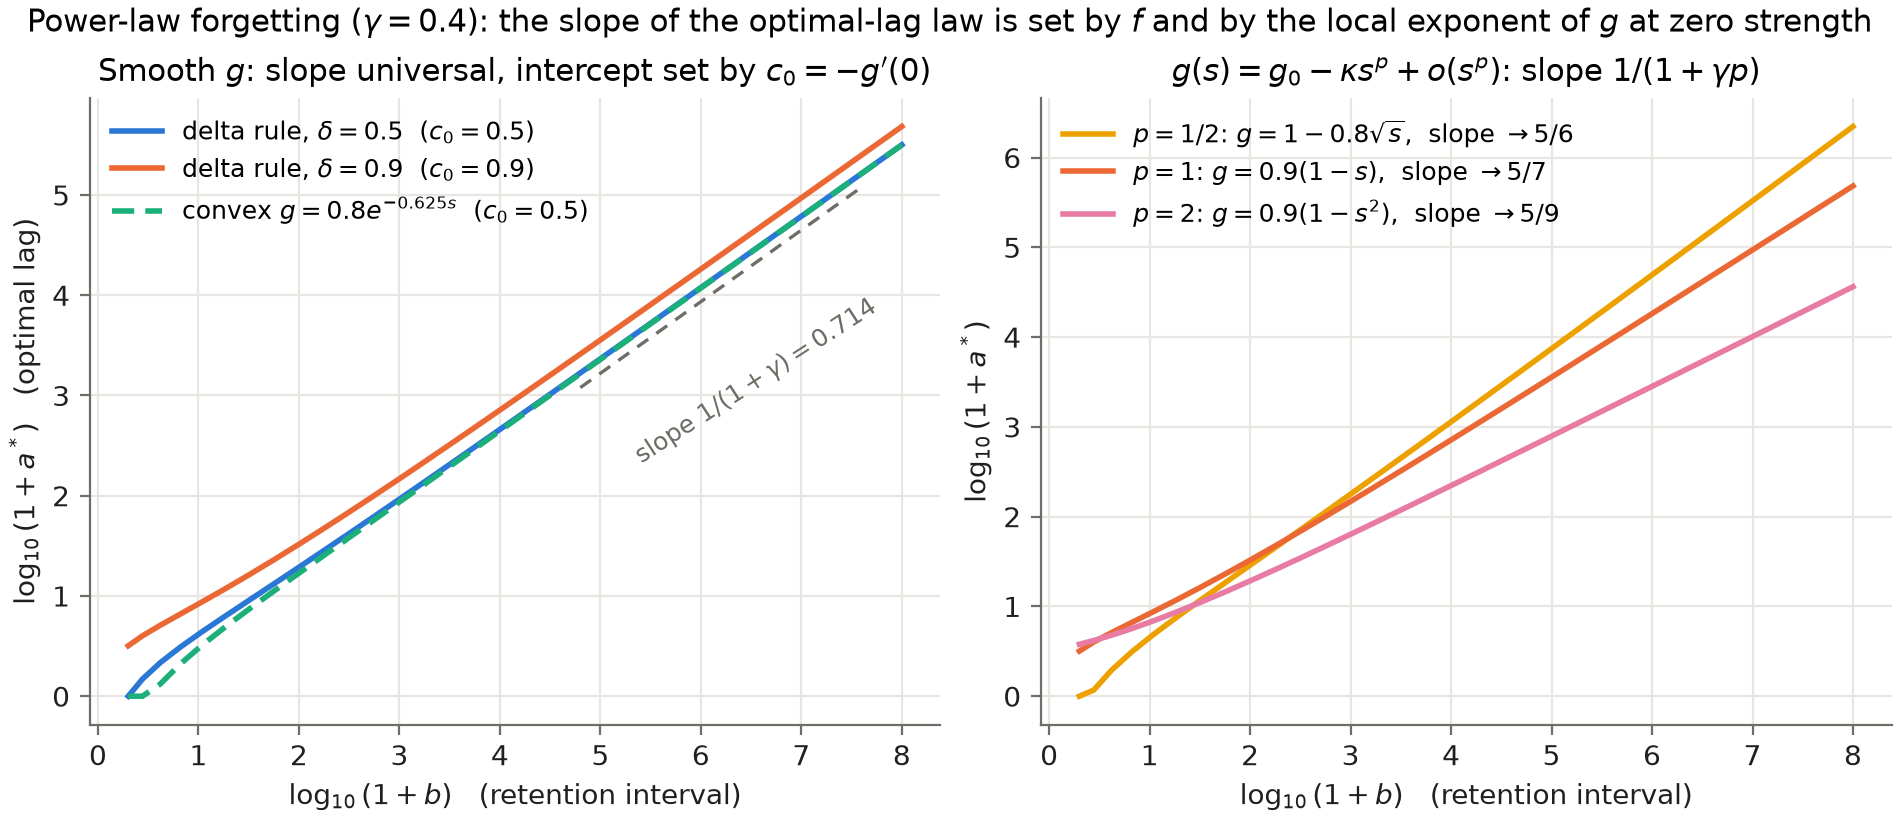
\includegraphics[width=1\linewidth]{figures/f3_general_universality.png}
  \caption{Numerical verification of Theorem~\ref{thm:universal} and Remark~\ref{rem:classes} with power-law forgetting ($\gamma=0.4$; brute-force maximization of Equation~\ref{eq:S}). Left: three different smooth learning functions produce parallel optimal-lag lines with the universal slope $1/(1+\gamma)$ (dashed guide); the learning function moves only the intercept, through $c_0=-g'(0)$, so the convex function with $c_0=0.5$ (dashed) converges onto the delta rule with $\delta=0.5$. Right: learning functions with local exponent $p$ at zero strength ($g \approx g_0 - \kappa s^p$) produce slope $1/(1+\gamma p)$.}\label{fig:general-universality}
\end{figure}

\subsection{The Long-Delay Fate of the Optimal Lag: a Tail Trichotomy}

Power-law decay is sufficient for the empirical profile, but what exactly is necessary? The long-retention-interval behavior of the optimal lag is decided by the \emph{tail hazard} of forgetting.

\begin{theorem}[Tail trichotomy]\label{thm:tails}
Let $g$ be suppressive, $h(0)>0$, and let $f$ in addition be convex (so $m$ is nonincreasing).
(i) If $h(t) \to 0$ as $t \to \infty$ (subexponential tail; e.g., any power law), then every maximizer branch satisfies $a^*(b) \to \infty$.
(ii) If $f(t) = w e^{-r t}\big(1+o(1)\big)$ and $m(t) = w r e^{-r t}\big(1+o(1)\big)$ for some $w \in (0,1]$, $r>0$ (exponential tail; e.g., any finite mixture $\sum_i w_i e^{-r_i t}$ with $r = \min_i r_i$), and the equation
\begin{equation}\label{eq:sat}
  c\big(g_0 f(a)\big)\, m(a) \;=\; r\, e^{-r a}
\end{equation}
has a unique, transversal root $a_\infty$, then $a^*(b) \to a_\infty < \infty$: the optimal lag \emph{saturates}.
(iii) If $h(t) \to \infty$ (superexponential tail), massed restudy is locally optimal at all sufficiently long retention intervals.
\end{theorem}

\begin{proof}[Proof sketch]
(i) If $a^*$ were bounded along a subsequence, the first-order condition (Equation~\ref{eq:foc}) would give $C(a^*)\, m(a^*) = m(a^*+b)/f(b) \leq m(b)/f(b) = h(b) \to 0$ (using $m$ nonincreasing), contradicting that $C\,m$ is continuous and positive on compact lag sets. (An interior optimum exists for large $b$ because $h(b)\to 0 < c(g_0)h(0)$, Theorem~\ref{thm:onset}.)
(ii) Substituting the tail forms into Equation~\ref{eq:foc}, the factors $w e^{-rb}$ cancel and the condition converges to Equation~\ref{eq:sat}; transversality gives convergence of the root.
(iii) is Theorem~\ref{thm:onset}(ii).
\end{proof}

\begin{remark}[Trace heterogeneity buys the pattern]\label{rem:mixtures}
The trichotomy has a substantive reading. Suppose each trace is made of components decaying exponentially at heterogeneous rates, so that $f$ is a mixture $f(t) = \int e^{-r t}\, d\mu(r)$ (a completely monotone function). A degenerate $\mu$ (pure exponential) yields a retention-interval-independent optimal lag (Theorem~\ref{thm:exp}); a finite mixture yields an optimal lag that rises but saturates at a ceiling tied to its slowest decay rate (Theorem~\ref{thm:tails}(ii)); and scale-free rate heterogeneity --- e.g., Gamma-distributed rates, which give exactly $f(t) = (1+t/\theta)^{-\gamma}$ --- yields the unbounded, log-log-linear growth of Theorem~\ref{thm:universal}. In this precise sense the Cepeda pattern is a signature of \emph{multi-timescale} forgetting (cf. Anderson \& Schooler 1991; Staddon, Chelaru, \& Higa 2002; Mozer et al. 2009), not of any particular learning rule. Figure~\ref{fig:general-tails} (left) shows all three fates under one and the same learning function.
\end{remark}

\begin{figure}
  \centering
  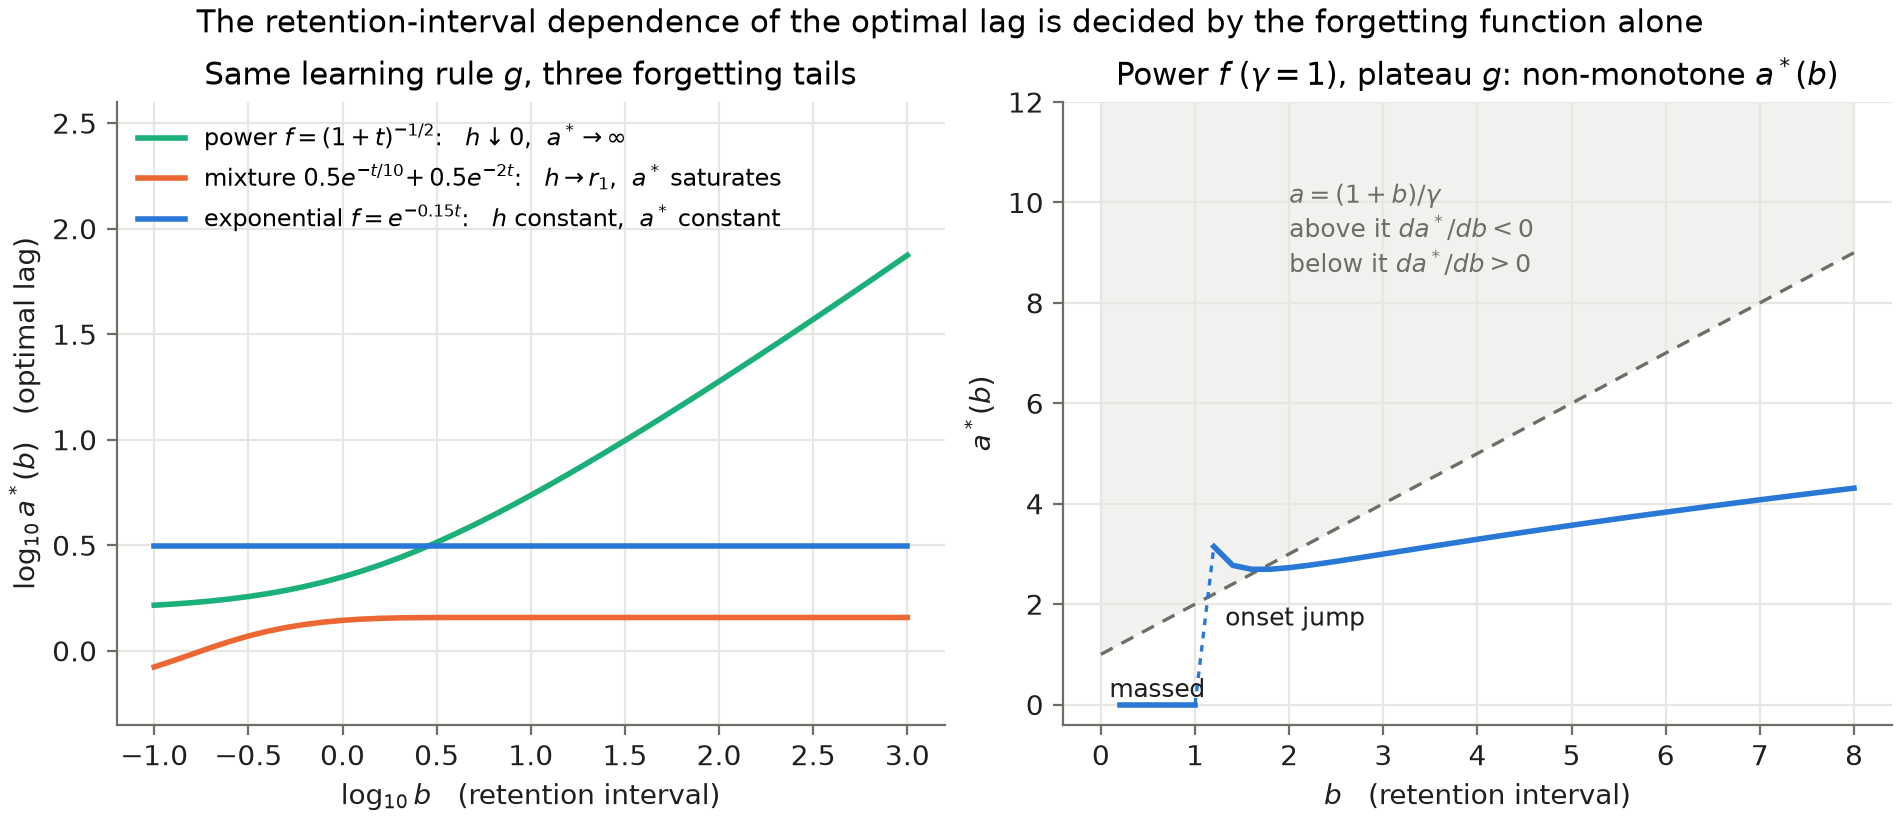
\includegraphics[width=1\linewidth]{figures/f4_general_forgetting_tails.png}
  \caption{The retention-interval dependence of the optimal lag is decided by the forgetting function alone. Left: brute-force optimal lag $a^*(b)$ under one fixed concave learning function $g(s) = 2 - 0.5s - 0.2s^2$ and three forgetting functions: constant hazard (exponential) gives a constant optimal lag (Theorem~\ref{thm:exp}); a two-exponential mixture gives a lag that saturates at the root of Equation~\ref{eq:sat} (Theorem~\ref{thm:tails}); a power law gives unbounded growth (Theorem~\ref{thm:universal}). Right: the sign rule (Theorem~\ref{thm:sign}, Corollary~\ref{cor:signpower}) at work for power-law forgetting ($\gamma = 1$) with a steep-then-flat learning function $g(s) = 1 - \frac{1.9}{1.5}(1-e^{-1.5 s})$: the optimum onsets discontinuously above the line $a=(1+b)/\gamma$, decreases while above it, and increases after crossing into the absorbing region below (Theorem~\ref{thm:power}(ii)).}\label{fig:general-tails}
\end{figure}

\subsection{Numerical Verification}

All claims were verified by brute-force maximization of Equation~\ref{eq:S} over fine lag grids, independent of the calculus (\texttt{src/spacing-general-verification.py}; ten checks). In particular: the onset threshold $b_c$ is exact; under exponential decay the maximizer is constant across four orders of magnitude of $b$ and equals $f^{-1}(s^*/g_0)$ with $c(s^*)=1$; the delta-rule closed form (Equation~\ref{eq:closedform}) matches the brute-force optimum, which is strictly increasing and confined below $a=(1+b)/\gamma$; the counterexample of Corollary~\ref{cor:signpower} decreases exactly while above that line; fitted log-log slopes match $1/(1+\gamma p)$ within $0.02$ for five learning functions with $p \in \{1/2, 1, 2\}$; the asymptotic constants converge to $\kappa p g_0^{p-1}$; and the two-exponential mixture saturates at the root of Equation~\ref{eq:sat} to four decimals.

\subsection{Summary: the General Theorems}

For the two-repetition model of Equation~\ref{eq:S}, the mapping from empirical properties to model ingredients is:
\begin{center}
\begin{tabular}{p{0.44\linewidth} p{0.5\linewidth}}
\hline
\textbf{Property of the data} & \textbf{Characterization} \\
\hline
Spacing beats massed at retention interval $b$ & $h(b) < c(g_0)\, h(0)$ (Theorem~\ref{thm:onset}); requires suppressive learning, $g' < 0$ (Proposition~\ref{prop:suppression}) \\
Optimal lag depends on $b$ at all & $f$ non-exponential; exponential decay is the exactly separable knife edge (Theorem~\ref{thm:exp}) \\
Direction of the lag $\times$ retention-interval interaction & $\operatorname{sign}(da^*/db) = \operatorname{sign}[\lambda(a^*+b) - h(b)]$: a property of forgetting alone (Theorem~\ref{thm:sign}) \\
Optimal lag increasing over the whole range & power law + concave $g$: exact; any suppressive $g$: eventually (Theorem~\ref{thm:power}) \\
Log-log linear, slope $\sigma \in (0,1)$, parameter changes shift only the intercept & power-type tail; $\sigma = 1/(1+\gamma)$ universally over smooth $g$; $g$ enters only via $c_0 = -g'(0)$ (Theorem~\ref{thm:universal}) \\
Optimal lag unbounded vs.\ saturating vs.\ constant in $b$ & tail hazard $h(\infty) = 0$ vs.\ $h(\infty) > 0$ vs.\ $h$ constant (Theorem~\ref{thm:tails}) \\
\hline
\end{tabular}
\end{center}

Two further one-line consequences are worth recording. First, by the envelope theorem, peak performance still declines with the retention interval, $\frac{d}{db} S(a^*(b), b) = g_0 f'(a^*+b) + g(s_{a^*}) f'(b) < 0$, as in the data. Second, the identification corollary cuts both ways: given the meta-analytic slope, the forgetting exponent is not a free parameter, and given a forgetting exponent measured from retention curves, the position and slope of the optimal-lag line are parameter-free predictions up to the single intercept constant $c_0$.

In short, the most general statement supported by the model family of Equation~\ref{eq:S} is this: \emph{any} suppressive learning function paired with \emph{any} decelerating (decreasing-hazard, vanishing-tail-hazard) forgetting function reproduces the qualitative Cepeda profile beyond a short-interval threshold; the quantitative log-log law, its slope, and its parameter-invariance are properties of power-law-type forgetting and of nothing else; and both the constancy of the optimal lag under exponential decay and the impossibility of a spacing effect without suppression are exact characterizations, not artifacts of the delta rule.

%\section{General Discussion}

%\printbibliography

\end{document}
